\documentclass[portrait,a0paper,fontscale=0.315]{baposter}

\usepackage{calc}
\usepackage{graphicx}
\usepackage{amsmath}
\usepackage{amssymb}
\usepackage{relsize}
\usepackage{multirow}
\usepackage{rotating}
\usepackage{bm}
\usepackage{url}
\usepackage{graphicx}
\usepackage{multicol}
\usepackage{enumitem}
\usepackage[export]{adjustbox}% http://ctan.org/pkg/adjustbox

%\usepackage{times}
%\usepackage{helvet}
%\usepackage{bookman}
\usepackage{palatino}

\newcommand{\captionfont}{\footnotesize}

\graphicspath{{images/}{../images/}}
\usetikzlibrary{calc}

%%%%%%%%%%%%%%%%%%%%%%%%%%%%%%%%%%%%%%%%%%%%%%%%%%%%%%%%%%%%%%%%%%%%%%%%%%%%%%%%
%%%% Some math symbols used in the text
%%%%%%%%%%%%%%%%%%%%%%%%%%%%%%%%%%%%%%%%%%%%%%%%%%%%%%%%%%%%%%%%%%%%%%%%%%%%%%%%

%%%%%%%%%%%%%%%%%%%%%%%%%%%%%%%%%%%%%%%%%%%%%%%%%%%%%%%%%%%%%%%%%%%%%%%%%%%%%%%%
% Multicol Settings
%%%%%%%%%%%%%%%%%%%%%%%%%%%%%%%%%%%%%%%%%%%%%%%%%%%%%%%%%%%%%%%%%%%%%%%%%%%%%%%%
\setlength{\columnsep}{1.5em}
\setlength{\columnseprule}{0mm}

%%%%%%%%%%%%%%%%%%%%%%%%%%%%%%%%%%%%%%%%%%%%%%%%%%%%%%%%%%%%%%%%%%%%%%%%%%%%%%%%
% Save space in lists. Use this after the opening of the list
%%%%%%%%%%%%%%%%%%%%%%%%%%%%%%%%%%%%%%%%%%%%%%%%%%%%%%%%%%%%%%%%%%%%%%%%%%%%%%%%
\newcommand{\compresslist}{%
\setlength{\itemsep}{1pt}%
\setlength{\parskip}{0pt}%
\setlength{\parsep}{0pt}%
}

\begin{document}
\begin{poster}%
  % Poster Options
  {
  % Show grid to help with alignment
  grid=false,
  % Column spacing
  colspacing=1em,
  % Color style
  bgColorOne=white,
  bgColorTwo=white,
  borderColor=black,
  headerColorOne=red,
  headerColorTwo=red,
  headerFontColor=white,
  boxColorOne=white,
  % Format of textbox
  textborder=roundedleft,
  % Format of text header
  eyecatcher=true,
  headerborder=closed,
  headerheight=0.135\textheight,
%  textfont=\sc, An example of changing the text font
  headershape=roundedright,
  headershade=shadelr,
  headerfont=\Large\bf\textsc, %Sans Serif
  textfont={\setlength{\parindent}{1.5em}},
  boxshade=plain,
%  background=shade-tb,
  background=plain,
  linewidth=2pt
  }
  % Group logo
  {\includegraphics[height=7.0em]{images/rambaut_group_logo}} 
  % Title
  {\bf\textsc{Phylodynamics of Ebola Virus in West Africa\linespread{0.25}\par}\vspace{0.25em}}
  % Authors
  {\textsc{Luiz Max de Carvalho$^{1,}$\footnote{{\small \texttt{lm.carvalho@ed.ac.uk}\\ $^1$ Institute of Evolutionary Biology, University of Edinburgh, UK.\\ Supervisors: Andrew Rambaut and Darren Obbard.}}}\\}
  % University logo
   { \includegraphics[height=7.0em]{images/edi_logo}}
%%%%%%%%%%%%%%%%%%%%%%%%%%%%%%%%%%%%%%%%%%%%%%%%%%%%%%%%%%%%%%%%%%%%%%%%%%%%%%
\headerbox{Background}{name=problem,column=0,row=0}{
%%%%%%%%%%%%%%%%%%%%%%%%%%%%%%%%%%%%%%%%%%%%%%%%%%%%%%%%%%%%%%%%%%%%%%%%%%%%%%
 \subsubsection*{Mode and tempo of the epidemic}
The 2013-2016 West African Ebola virus disease (EVD) epidemic was the largest in history.
A massive international collaboration produced the most comprehensive data set for an acute virus to date (over 5\% sampling).
Detailed information about viral movement in West Africa using $1610$ viral genomes was recently made available (Dudas et al. (2016)).
A major challenge is to develop the statistical and computational tools to combine different sources of information (epidemiological, genetic, climatic, etc) to trace the epidemic and explain its mode and \texit{tempo}.
Which climatic and socio-economic factors predict outbreak sizes? 
\subsubsection*{Association between a particular mutation and disease severity}
There is experimental evidence that an A$\rightarrow$V mutation in the glycoprotein (GP) confers increased infectivity in human cells.
I investigate the association between GP82-AV and disease severity using $236$ genomes for which clinical metadata was available.
}
%%%%%%%%%%%%%%%%%%%%%%%%%%%%%%%%%%%%%%%%%%%%%%%%%%%%%%%%%%%%%%%%%%%%%%%%%%%%%%%%%
%%%%%%%%%%%%%%%%%%%%%%%%%%%%%%%%%%%%%%%%%%%%%%%%%%%%%%%%%%%%%%%%%%%%%%%%%%%%%%%%%
\headerbox{Results}{name=results,column=1,span=2,row=0}{
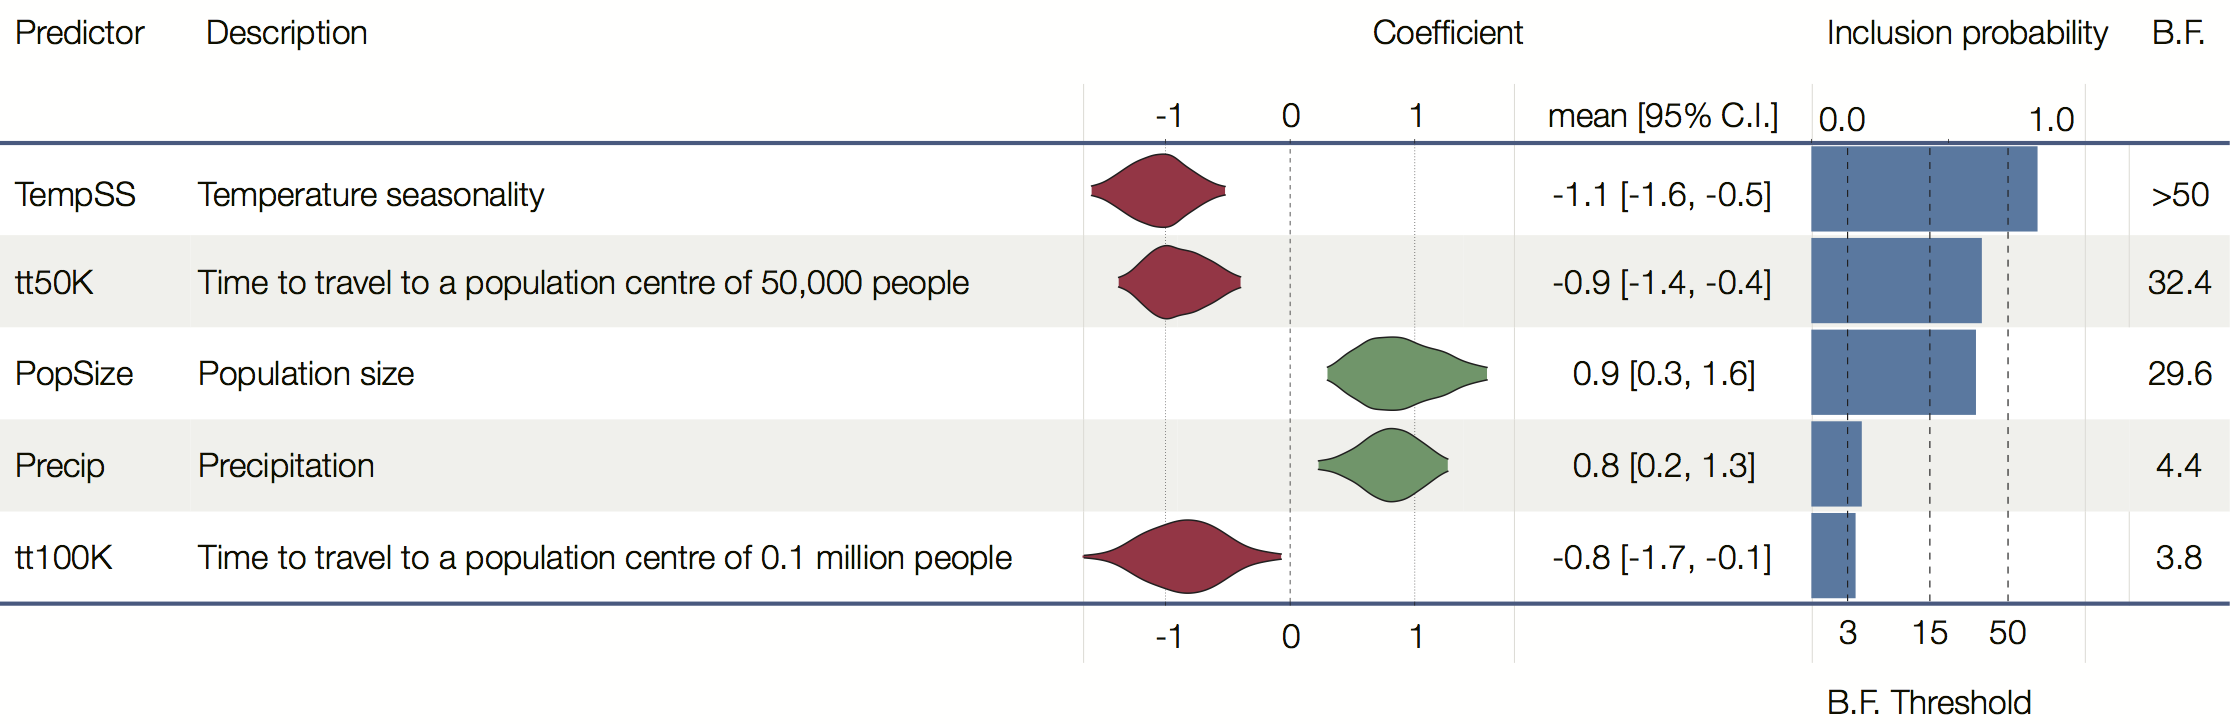
\includegraphics[scale=0.19,valign=c]{images/case-count_coefficients.png}\\
\textbf{Predictors of EVD outbreak sizes in West Africa}.
We show the predictors with Bayes factor (BF) greater than 3.
We find that low temperature seasonality and higher levels of rain increase the risk of larger outbreaks.
Similarly, urbanicity seems to play a role, with locations closer to urban centres having more cases (controlling for population sizes).\\
\\
%%%%%%%%%%%%%%%%%%%%%%%%%%%%%%%%%%%%%%%%%%%%%%%%%%%%%%%%%%%%%%%%%%%%%%%%%%%%%%%%%
 \begin{tabular}{cc}
 \includegraphics[scale=0.1,valign=c]{images/EVD_traits_tree.png} &
 \includegraphics[scale=0.35,valign=c]{images/predicted_fatality_rates.pdf}
\end{tabular} \\
\\
\textbf{Association between the GP82-AV and disease severity.}
The left panel shows a time-calibrated phylogeny with 236 sequences from patients whose outcome information was available.
Branches with lower viral loads (transformed $C_t$) have higher probability of leading to cases where the patient survived, suggesting some degree of heritability of infectivity.
The right panel shows the predicted fatality rates conditional on viral load for each genotype (wild type: \textbf{A}, mutant: \textbf{V}).
Notice that although fatality rates seem be higher for \textbf{V} the confidence bands overlap considerably, indicating substantial uncertainty.\\
\\
%%%%%%%%%%%%%%%%%%%%%%%%%%%%%%%%%%%%%%%%%%%%%%%%%%%%%%%%%%%%%%%%%%%%%%%%%%%%%%%%%% 
\begin{tabular}{ccc}
 \includegraphics[scale=0.34,valign=c]{images/maxCases_Dubreka.png} &
 \includegraphics[scale=0.34,valign=c]{images/maxCases_Kailahun.png}&
 \includegraphics[scale=0.34,valign=c]{images/maxCases_Gueckedou.png}
\end{tabular}\\

\textbf{Combining epidemiological and genetic data}.
Here weekly recorded cases for three representative locations are overlaid with inferred introductions to gain insight into the dynamics of EVD the epidemic.
Dashed vertical line marks the earliest introduction in the posterior.
Tick marks at the top show the dates of sampling of the sequences in that location.

\section*{Conclusions}
\begin{itemize}
 \item Both climatic and social economic factors predict outbreak sizes.
 We have employed this approach to help explain why some regions did not experience cases despite being in close proximity with affected areas.
 \item The A$\rightarrow$V mutation in the EBOV glycoprotein is weakly associated with higher fatality rates;
 \item By combining epidemiological information and viral movement inferred from sequenced genomes one can gain insight into the dynamics of Ebola in West Africa.
 Our challenge now is to integrate all of this information in a coherent statistical model.
\end{itemize}

Funding: I thank the Principal's Career Development Scholarship and the School of Biological Sciences funding my PhD.
}
%%%%%%%%%%%%%%%%%%%%%%%%%%%%%%%%%%%%%%%%%%%%%%%%%%%%%%%%%%%%%%%%%%%%%%%%%%%%%%
\headerbox{Methods}{name=method,column=0,below=problem}{
%%%%%%%%%%%%%%%%%%%%%%%%%%%%%%%%%%%%%%%%%%%%%%%%%%%%%%%%%%%%%%%%%%%%%%%%%%%%%%
Weekly reported cases were available for $56$ locations.
For $236$ cases complete metadata, including $C_t$ values and outcome (death/survival) information was available.
$C_t$ stands for ``threshold cycle'' and records the number of qPCR cycles required to to detect a real signal from the samples.
These values are inversely correlated with viral load.
Using $1610$ genomes, Dudas et al. (2016) inferred how many viral introductions each location received, and how many samples resulted from each introduction.
\begin{itemize}[leftmargin=*]
 \item[$\oint$] Let  $Y_i$ be total number of cases reported for location $i$. 
Let also $\mathbf{X_i}$ be a set of $P$ climatic and socio-economic covariates measured at location $i$.
I then employ a negative binomial generalised linear model (GLM) coupled with stochastic search variable selection:
\begin{align*}
 Y_i & \sim \text{NegBin}(p_i, r) \\
 p_i & = \frac{r}{(r + \lambda_i)}  \\ 
\log(\lambda_i) &= \alpha + \beta_{1}\delta_{1} x_{i1} + \ldots + \beta_{P}\delta_{P} x_{iP} 
\end{align*}
This approach has the advantage of allowing for the calculation of Bayes factors (BF) analytically.
Let $w_0$ be the (prior) probability that no predictors are included. 
Then the Bayes factor supporting predictor $x_j$ is
\begin{equation*}
 \text{BF}(x_j) = \frac{\hat{\delta_j}w_0^{1/P}}{(1-\hat{\delta_j})(1 - w_0^{1/P})}
\end{equation*}
where $\hat{\delta_j}$ is the posterior inclusion probability.
%%%%%%%%%%%%%%%%%%%%%%%%%%%%%%%%%%%%%%%%%%%%%%%%%
 \item[$\oint$]  To use $C_t$ values as a proxy for viral load and also consistent with the mutation (binary) predictor we standardise $C_t$ by subtracting from the mean and dividing by two standard deviations.
 I then fit a binomial GLM using outcome as response variable and the absence/presence of the mutation and $C_t$ values as covariates.
%%%%%%%%%%%%%%%%%%%%%%%%%%%%%%%%%%%%%%%%%%%%%%%%%
 \item[$\oint$] Constructing outbreak clusters: every time a location receives a viral introduction that leads to $>$20 sampled cases, split the series before and after the introduction.
\end{itemize}
}
\end{poster}
\end{document}